% This file was converted to LaTeX by Writer2LaTeX ver. 1.0.2
% see http://writer2latex.sourceforge.net for more info
\documentclass[12pt]{article}
\usepackage[utf8]{inputenc}
\usepackage[T1]{fontenc}
\usepackage[english]{babel}
\usepackage{amsmath}
\usepackage{amssymb,amsfonts,textcomp}
\usepackage{array}
\usepackage{supertabular}
\usepackage{hhline}
\usepackage{hyperref}
\hypersetup{colorlinks=true, linkcolor=blue, citecolor=blue, filecolor=blue, urlcolor=blue}
\usepackage{graphicx}
% Text styles
\newcommand\textstyleListLabellv[1]{\textrm{#1}}
\newcommand\textstyleListLabellvi[1]{#1}
\newcommand\textstylefootnotereference[1]{{\fontsize{6.5pt}{7.8pt}\selectfont #1}}
\makeatletter
\newcommand\arraybslash{\let\\\@arraycr}
\makeatother
\raggedbottom
% Paragraph styles
\renewcommand\familydefault{\rmdefault}
\newenvironment{styleStandard}{\setlength\leftskip{0cm}\setlength\rightskip{0cm plus 1fil}\setlength\parindent{0cm}\setlength\parfillskip{0pt plus 1fil}\setlength\parskip{0in plus 1pt}\writerlistparindent\writerlistleftskip\leavevmode\normalfont\normalsize\writerlistlabel\ignorespaces}{\unskip\vspace{0.111in plus 0.0111in}\par}
\newenvironment{stylelsAbstract}{\setlength\leftskip{0.5in}\setlength\rightskip{0.5in}\setlength\parindent{0in}\setlength\parfillskip{0pt plus 1fil}\setlength\parskip{0in plus 1pt}\writerlistparindent\writerlistleftskip\leavevmode\normalfont\normalsize\itshape\writerlistlabel\ignorespaces}{\unskip\vspace{0.111in plus 0.0111in}\par}
\newenvironment{stylelsSectioni}{\setlength\leftskip{0.25in}\setlength\rightskip{0in plus 1fil}\setlength\parindent{0in}\setlength\parfillskip{0pt plus 1fil}\setlength\parskip{0.1665in plus 0.016649999in}\writerlistparindent\writerlistleftskip\leavevmode\normalfont\normalsize\fontsize{18pt}{21.6pt}\selectfont\bfseries\writerlistlabel\ignorespaces}{\unskip\vspace{0.0835in plus 0.00835in}\par}
\newenvironment{stylelsSectionii}{\setlength\leftskip{0.25in}\setlength\rightskip{0in plus 1fil}\setlength\parindent{0in}\setlength\parfillskip{0pt plus 1fil}\setlength\parskip{0.222in plus 0.0222in}\writerlistparindent\writerlistleftskip\leavevmode\normalfont\normalsize\fontsize{16pt}{19.2pt}\selectfont\bfseries\writerlistlabel\ignorespaces}{\unskip\vspace{0.0835in plus 0.00835in}\par}
\newenvironment{styleListParagraph}{\setlength\leftskip{0.5in}\setlength\rightskip{0in plus 1fil}\setlength\parindent{0in}\setlength\parfillskip{0pt plus 1fil}\setlength\parskip{0in plus 1pt}\writerlistparindent\writerlistleftskip\leavevmode\normalfont\normalsize\writerlistlabel\ignorespaces}{\unskip\vspace{0.111in plus 0.0111in}\par}
% List styles
\newcommand\writerlistleftskip{}
\newcommand\writerlistparindent{}
\newcommand\writerlistlabel{}
\newcommand\writerlistremovelabel{\aftergroup\let\aftergroup\writerlistparindent\aftergroup\relax\aftergroup\let\aftergroup\writerlistlabel\aftergroup\relax}
\newcounter{listWWNumxxiileveli}
\newcounter{listWWNumxxiilevelii}[listWWNumxxiileveli]
\newcounter{listWWNumxxiileveliii}[listWWNumxxiilevelii]
\newcounter{listWWNumxxiileveliv}[listWWNumxxiileveliii]
\renewcommand\thelistWWNumxxiileveli{\arabic{listWWNumxxiileveli}}
\renewcommand\thelistWWNumxxiilevelii{\arabic{listWWNumxxiileveli}.\arabic{listWWNumxxiilevelii}}
\renewcommand\thelistWWNumxxiileveliii{\arabic{listWWNumxxiileveli}.\arabic{listWWNumxxiilevelii}.\arabic{listWWNumxxiileveliii}}
\renewcommand\thelistWWNumxxiileveliv{\arabic{listWWNumxxiileveli}.\arabic{listWWNumxxiilevelii}.\arabic{listWWNumxxiileveliii}.\arabic{listWWNumxxiileveliv}}
\newcommand\labellistWWNumxxiileveli{\thelistWWNumxxiileveli.}
\newcommand\labellistWWNumxxiilevelii{\thelistWWNumxxiilevelii.}
\newcommand\labellistWWNumxxiileveliii{\thelistWWNumxxiileveliii.}
\newcommand\labellistWWNumxxiileveliv{\thelistWWNumxxiileveliv.}
\newenvironment{listWWNumxxiileveli}{\def\writerlistleftskip{\addtolength\leftskip{0.0cm}}\def\writerlistparindent{}\def\writerlistlabel{}\def\item{\def\writerlistparindent{\setlength\parindent{-0cm}}\def\writerlistlabel{\stepcounter{listWWNumxxiileveli}\makebox[0cm][l]{\labellistWWNumxxiileveli}\hspace{0cm}\writerlistremovelabel}}}{}
\newenvironment{listWWNumxxiilevelii}{\def\writerlistleftskip{\addtolength\leftskip{0.0cm}}\def\writerlistparindent{}\def\writerlistlabel{}\def\item{\def\writerlistparindent{\setlength\parindent{-0cm}}\def\writerlistlabel{\stepcounter{listWWNumxxiilevelii}\makebox[0cm][l]{\labellistWWNumxxiilevelii}\hspace{0cm}\writerlistremovelabel}}}{}
\newenvironment{listWWNumxxiileveliii}{\def\writerlistleftskip{\addtolength\leftskip{0.0cm}}\def\writerlistparindent{}\def\writerlistlabel{}\def\item{\def\writerlistparindent{\setlength\parindent{-0cm}}\def\writerlistlabel{\stepcounter{listWWNumxxiileveliii}\makebox[0cm][r]{\labellistWWNumxxiileveliii}\hspace{0cm}\writerlistremovelabel}}}{}
\newenvironment{listWWNumxxiileveliv}{\def\writerlistleftskip{\addtolength\leftskip{0.0cm}}\def\writerlistparindent{}\def\writerlistlabel{}\def\item{\def\writerlistparindent{\setlength\parindent{-0cm}}\def\writerlistlabel{\stepcounter{listWWNumxxiileveliv}\makebox[0cm][l]{\labellistWWNumxxiileveliv}\hspace{0cm}\writerlistremovelabel}}}{}
\newcommand\labellistWWNumxxxiiileveli{\textstyleListLabellv{o}}
\newcommand\labellistWWNumxxxiiilevelii{\textstyleListLabellvi{o}}
\newcommand\labellistWWNumxxxiiileveliii{[F0A7?]}
\newcommand\labellistWWNumxxxiiileveliv{[F0B7?]}
\newenvironment{listWWNumxxxiiileveli}{\def\writerlistleftskip{\addtolength\leftskip{0.0cm}}\def\writerlistparindent{}\def\writerlistlabel{}\def\item{\def\writerlistparindent{\setlength\parindent{-0cm}}\def\writerlistlabel{\makebox[0cm][l]{\labellistWWNumxxxiiileveli}\hspace{0cm}\writerlistremovelabel}}}{}
\newenvironment{listWWNumxxxiiilevelii}{\def\writerlistleftskip{\addtolength\leftskip{0.0cm}}\def\writerlistparindent{}\def\writerlistlabel{}\def\item{\def\writerlistparindent{\setlength\parindent{-0cm}}\def\writerlistlabel{\makebox[0cm][l]{\labellistWWNumxxxiiilevelii}\hspace{0cm}\writerlistremovelabel}}}{}
\newenvironment{listWWNumxxxiiileveliii}{\def\writerlistleftskip{\addtolength\leftskip{0.0cm}}\def\writerlistparindent{}\def\writerlistlabel{}\def\item{\def\writerlistparindent{\setlength\parindent{-0cm}}\def\writerlistlabel{\makebox[0cm][l]{\labellistWWNumxxxiiileveliii}\hspace{0cm}\writerlistremovelabel}}}{}
\newenvironment{listWWNumxxxiiileveliv}{\def\writerlistleftskip{\addtolength\leftskip{0.0cm}}\def\writerlistparindent{}\def\writerlistlabel{}\def\item{\def\writerlistparindent{\setlength\parindent{-0cm}}\def\writerlistlabel{\makebox[0cm][l]{\labellistWWNumxxxiiileveliv}\hspace{0cm}\writerlistremovelabel}}}{}
\setlength\tabcolsep{1mm}
\renewcommand\arraystretch{1.3}
% footnotes configuration
\makeatletter
\renewcommand\thefootnote{\arabic{footnote}}
\makeatother
\title{}
\author{UIC}
\date{2018-01-17}
\begin{document}
\title{\textsuperscript{Exploring the acquisition of countable and uncountable nouns }\newline
in EMI and FI contexts}
\maketitle

\begin{styleStandard}
\textit{Dakota J. Thomas-Wilhelm, University of Iowa / Universitat Autònoma de Barcelona; }\textit{Carmen Pérez-Vidal, Universitat Pompeu Fabra}
\end{styleStandard}

\begin{stylelsAbstract}
The present study aims at exploring the acquisition and mental representation of the countable and uncountable noun distinction in English as a foreign language (EFL) by two upper-intermediate Catalan/Spanish groups in two different learning contexts, formal instruction (FI) and English-Medium Instruction (EMI) (Coleman 2006; Izumi 2013), in contrast with baseline native speaker data, and with an interest in crosslinguistic influence. The FI group receives fewer hours of exposure to EFL, 3 per week, but in return, instruction on the phenomenon under study. In contrast, the EMI group is immersed in EFL, receiving 15-20 hours per week in the classroom, but receives no instruction on the phenomenon in question. Data were collected by means of four experimental tasks: one grammaticality judgment task and three picture-decision tasks. The results show that, although there is no significant difference between learning context overall, there are differences when the data are considered at the level of the noun-type. The lack of impact resulting from FI adds further evidence to the existing discussion related to explicit (FI) versus implicit (EMI) instructional contexts (Dafouz Milne \& Guerrini 2009; Pérez-Vidal 2009; 2011). In addition, these findings underscore the difficulty in the acquisition of countable and uncountable noun type distinctions at upper-intermediate levels. 
\end{stylelsAbstract}

\setcounter{listWWNumxxiileveli}{0}
\begin{listWWNumxxiileveli}
\item 
\begin{stylelsSectioni}
Introduction
\end{stylelsSectioni}

\end{listWWNumxxiileveli}
\begin{styleStandard}
At the intersection of semantics, syntax, and language acquisition is ongoing research about how semantics and syntax are related, and an extension of that is the question of how \ language learners acquire this relationship. Barner \& Snedeker (2005: 42) pose a very important question: “how [does] the knowledge in one domain facilitate [the] acquisition of knowledge in the other?” The relationship between countable and uncountable nouns is an exemplar of this relationship between semantics and syntax. This study focuses on how English as a Foreign language (EFL) learners from two different language acquisition contexts, Formal Instruction (FI) and English-Medium Instruction (EMI), acquire countability distinctions in their target language using both behavioral and cognitive data, with a Grammaticality Judgment Test (GJT) and a Picture Decision Task (PDT), respectively (Chaudron 2003; Norris \& Ortega 2003). The study presented in this chapter seeks to understand how EFL learners from each context comparatively recognize the countable/uncountable distinction and map it in their mental representations. 
\end{styleStandard}

\begin{styleStandard}
The study was conducted at a Catalan university, in Spain, where most of the subjects are taught in either Spanish or Catalan. However, following a relatively recent trend in Europe, English has increasingly become a third or additional language of instruction. Indeed, the so-called university EMI programs, modelled on similar programs existing at lower stages of education, have become current practice. Wächter \& Maiworm (2008) conducted a survey during the 2006/07 academic year to determine the number of EMI programs in the European Higher Education Area. Through their survey, they were able to identify 2,389 programs that were taught though English. These findings are remarkable and even more so as the trend was confirmed by a subsequent survey showing that 6\% of degrees in Europe would take an EMI approach (Wächter \& Maiworm 2014). 
\end{styleStandard}

\begin{listWWNumxxiileveli}
\item 
\begin{stylelsSectioni}
Literature Review
\end{stylelsSectioni}

\end{listWWNumxxiileveli}
\begin{styleStandard}
Expressing quantity is something that is common in every language. Although it is more complex and developed in some languages than others, nouns, noun phrases, and quantifiers/quantification all have very specific positions and functions in language that allow us to refer to things in both the real and abstract worlds. As can be seen in Table 1, English has five main subclasses of nouns that can refer to objects and substances with physical existence (Leech \& Svartvik 1975): (1) proper, (2) countable, (3) object-uncountable, (4) substance-uncountable, and (5) flexible. In the current study, we are only concerned with subclasses (2)-(5).
\end{styleStandard}

\begin{styleStandard}
\textit{Table 1: Noun subclasses in English}
\end{styleStandard}

\begin{flushleft}
\tablehead{}
\begin{supertabular}{m{0.42195985in}|m{1.0052599in}|m{1.0080599in}|m{1.0066599in}|m{1.0094599in}|m{1.0087599in}|}
\hline
\multicolumn{1}{|m{0.42195985in}|}{} &
\bfseries (1) Proper &
\bfseries (2) Countable &
\bfseries (3) Object-Uncountable &
\bfseries (4) Substance-Uncountable &
\bfseries (5) Flexible\\\hline
\multicolumn{1}{|m{0.42195985in}|}{\mdseries I see…} &
\mdseries John &
\mdseries *bottle &
\mdseries furniture &
\mdseries Salt &
\mdseries cake\\\hline
 &
\mdseries *the John &
\mdseries the bottle &
\mdseries the furniture &
\mdseries the salt &
\mdseries the cake\\\hhline{~-----}
 &
\mdseries *a John &
\mdseries a bottle &
\mdseries *a furniture &
\mdseries *a salt &
\mdseries a cake\\\hhline{~-----}
 &
\mdseries *some John &
\mdseries *some bottle &
\mdseries some furniture &
\mdseries some salt &
\mdseries some cake\\\hhline{~-----}
 &
\mdseries *Johns &
\mdseries bottles &
\mdseries *furnitures &
\mdseries *salts &
\mdseries cakes\\\hhline{~-----}
\end{supertabular}
\end{flushleft}
\begin{styleStandard}
In English, countable nouns refer to countable items and carry the semantic feature of [+\textit{count}] (and presumably [+ \textit{neat}]). On the contrary, uncountable nouns refer to non-countable items with the semantic feature [– \textit{count}], and may be [+ \textit{neat}] or [– \textit{neat}]. According to Landman (2011), a noun is [+ \textit{neat}] if the interpretation of its structures does not have overlapping minimal building blocks (e.g. \textit{furniture} is comprised of \textit{tables}, \textit{chairs}, \textit{sofas}, whereas a collection of just \textit{tables} would not be considered \textit{furniture}), and a noun is [– \textit{neat}] if it is comprised of multiple and similar parts which overlap (e.g. \textit{salt} is comprised of multiple, and similar,\textit{ grains of} \textit{salt}). On the basis of such a distinction, uncountable nouns are further divided into object-uncountable and substance-uncountable. Object-uncountable nouns are the nouns which are composed of objects (e.g. \textit{furniture, mail, luggage}) and carry the semantic features [– \textit{count}, + \textit{neat}], making them “neat” uncountable nouns since their interpretation does not have overlapping minimal building parts. On the other hand, substance-uncountable nouns (“messy” uncountable nouns), are those which have the semantic features [– \textit{count}, – \textit{neat}] and are composed of substances (e.g. \textit{salt, toothpaste, milk}), whose minimal building parts overlap. \ Lastly, flexible nouns are those which can be used as either countable or uncountable nouns [– \textit{count }/ + \textit{count}] (e.g. \textit{chocolate/chocolates}). In this respect, it is important to note that in the present study, we follow Barner \& Snedeker (2005) in positing that the interpretation of flexible nouns as one or the other is driven by the syntax in which they occur, i.e. in countable or uncountable syntactic constructions. This means that a flexible noun will be interpreted as either countable or uncountable given the context in which it appears. For example, if we compare the sentences \textit{I like chocolate }and \textit{She gave me two chocolates}, the quantifier \textit{two} in the latter sentence drives the interpretation of the flexible noun\textit{ chocolate} to being countable, while the use of the zero article, no quantifier, and singular form of the noun \textit{chocolate} drives the interpretation to be substance-uncountable in \textit{I like chocolate}, in the same way that \textit{salt }is uncountable in the sentence \textit{I need salt for my fries}.
\end{styleStandard}

\begin{styleStandard}
Spanish, Catalan and English largely overlap in the way they treat countable and uncountable nouns. Indeed, in the three languages countable nouns (like \textit{chair}) refer to countable items and mass-uncountable nouns (like \textit{water}) denote non-countable items (Bruyne 1995; Wheeler et al. 1999; Butt \& Benjamin 2004). The important difference is that some nouns that are treated as object-uncountable in English (thus appearing in the singular only in this language), \ in Spanish and Catalan have both a singular and plural form, expressing two different meanings. As can be seen in Tables 2 and 3, in Spanish or Catalan the singular form indicates an unspecified mass, while its plural refers to a plurality of objects; to express this meaning, English requires the addition of words that are countable elements. This is an important difference because one might expect that native speakers (NSs) of Spanish and Catalan might try to pluralize English uncountable nouns in trying to achieve the meaning that is similarly expressed in Spanish and Catalan.
\end{styleStandard}

\begin{styleStandard}
\textit{Table 2: }\textit{Pluralizing Spanish Uncountable Nouns}
\end{styleStandard}

\begin{flushleft}
\tablehead{}
\begin{supertabular}{m{1.1712599in}m{1.5906599in}|m{1.1712599in}m{1.5900599in}}
\hline
\multicolumn{2}{m{2.8406599in}|}{\bfseries SINGULAR} &
\multicolumn{2}{m{2.8400598in}}{\bfseries PLURAL}\\\hline
Spanish &
English &
Spanish &
English\\\hline
pan &
\textit{bread} &
panes &
\textit{loaves of bread}\\
tostada &
\textit{toast} &
tostadas &
\textit{pieces of toast}\\
equipaje &
\textit{luggage} &
equipajes &
\textit{pieces of luggage}\\
basura &
\textit{garbage} &
basuras &
\textit{bags of garbage}\\\hline
\end{supertabular}
\end{flushleft}
\begin{styleStandard}
\textit{Table 3: }\textit{Pluralizing Catalan Uncountable Nouns}
\end{styleStandard}

\begin{flushleft}
\tablehead{}
\begin{supertabular}{m{1.1504599in}m{1.5434599in}|m{1.2865599in}m{1.5427599in}}
\hline
\multicolumn{2}{m{2.7726598in}|}{\bfseries SINGULAR} &
\multicolumn{2}{m{2.90806in}}{\bfseries PLURAL}\\\hline
Catalan &
English &
Catalan &
English\\\hline
pa &
\textit{bread} &
pans &
\textit{loaves of bread}\\
torrada &
\textit{Toast} &
torrades &
\textit{pieces of toast}\\
equipatge &
\textit{Luggage} &
equipatges &
\textit{pieces of luggage}\\
basura &
\textit{garbage} &
basures &
\textit{bags of garbage}\\\hline
\end{supertabular}
\end{flushleft}
\begin{styleStandard}
From a developmental perspective, many hypotheses have been discussed about how children are sensitive to syntactic information when acquiring nouns that refer to collections of things in English (Bloom \& Keleman 1995). In the following paragraphs, we will describe the hypothesis put forth by Barner \& Snedeker (2005) and argue for how it may also apply to foreign language acquisition. 
\end{styleStandard}

\begin{styleStandard}
Barner \& Snedeker (2005) presented adults and 4-year old children with pictures and actual scenes, respectively, and asked the question \textit{Who has more?} One of the stimuli contained one or two large objects, the other three or six smaller objects, whose combined mass was clearly smaller than that of the other former object(s) (see Figure 2 for an example). All the four classes of nouns addressed in the present study were tested, viz. countable, object-uncountable, substance-uncountable, and flexible.
\end{styleStandard}

\begin{styleStandard}
Results show that, quite expectedly, both children and adults base their judgments on volume, or mass, for substance-uncountable nouns (e.g. a large chunk of \textit{toothpaste} is perceived as being ‘more’ than three small ones), and on number for countable nouns (e.g. three or six small \textit{shoes} are interpreted as ‘more \textit{shoes}’ than one or two big ones). The crucial finding was that both children and adults use number rather than mass in their judgments of object-uncountable nouns. Thus, three small \textit{chairs} and three small \textit{tables} are seen as being ‘more \textit{furniture}’ than a big table with a big chair. It thus seems that the inherent semantics of a word/concept like \textit{furniture} (which denotes a set of individual objects) overrides the lexico-syntactic constraints posed by a given language like English, which treats it as an uncountable noun like \textit{water}. 
\end{styleStandard}

\begin{styleStandard}
However, syntax does play a role in the case of flexible nouns, like \textit{string}. Here, a plural syntactic context like \textit{Who has more strings?} causes most participants to choose the picture with several small pieces of string, whereas a singular syntactic context like \textit{Who has more string?} led to choosing that with a long piece of string. 
\end{styleStandard}

\begin{styleStandard}
Thus, ‘individuation’, i.e. the interpretation of a term as referring to an individual or a collection of individuals, can have at least three sources: inherent semantics, or world knowledge (the fact that furniture or silverware represent, in the real world, a collection of objects); lexical features (the fact that, at least in English, ‘furniture’ and ‘silverware’ are singular-only nouns); and syntactic context (e.g. the presence of quantifiers and plural morphology, in the case of flexible nouns). 
\end{styleStandard}

\begin{listWWNumxxiileveli}
\item 
\begin{stylelsSectioni}
Methodology
\end{stylelsSectioni}

\end{listWWNumxxiileveli}
\begin{styleStandard}
These are the research questions addressed in the current study: 
\end{styleStandard}

\begin{styleStandard}
\textbf{RQ1. }How do FI learners compare to EMI learners, and to NSs, in their ability to grammatically recognize different countable/uncountable noun distinctions?
\end{styleStandard}

\begin{styleStandard}
\textbf{RQ2.} Are participants’ judgments about quantity based on linguistic knowledge or non-linguistic world-knowledge, and is there any difference in this regard among FI and EMI learners and native English speakers?? 
\end{styleStandard}

\begin{listWWNumxxiileveli}
\item 
\setcounter{listWWNumxxiilevelii}{0}
\begin{listWWNumxxiilevelii}
\item 
\begin{stylelsSectionii}
Participants
\end{stylelsSectionii}

\end{listWWNumxxiilevelii}
\end{listWWNumxxiileveli}
\begin{styleStandard}
A total of 57 participants completed the two experiments included in this study in order to address our two research questions. Of the 57 participants, 33 were undergraduates completing language-specialty degrees (FI group) and 24 were undergraduates studying business-related degrees through English (EMI group). These two groups were chosen because the FI undergraduates received explicit instruction in the English language, while the EMI only received implicit instruction since the content of their courses was taught through the medium of English. All participants were Spanish/Catalan simultaneous bilinguals from a public university in Catalonia, Spain. All participants were controlled for their level of English, on the basis of the Cambridge Online Placement Test of English. The group represented a relatively homogeneous population having an intermediate level, that is a B.1.2 according to the Common European Framework of Reference. However, results from this test revealed that the FI group had a relatively lower level (\textit{M }= 17.55, \textit{SD} = 3.80) than the EMI group (\textit{M }= 18.38, \textit{SD} = 0.57). As can be seen by the standard deviations, the FI group had considerable variation in level. An independent samples \textit{t}{}-test found that there was no significant difference in the English test scores for EMI and FI contexts (\textit{t}(34) = -1.235, \textit{p} = .225).
\end{styleStandard}

\begin{styleStandard}
In terms of target-language exposure, there are two main differences between the EMI and the FI group. Firstly, the students receiving EMI are receiving more hours per week of English language exposure than the FI group. The EMI group was receiving all of their classes in the degree, at that point, via EMI, which involves between 15-20 hours per week, according to the academic term. In contrast, the FI group only had a handful of classes that use English, for about \ three hours per week. Secondly, the FI class hours, as already mentioned, deal with grammar and linguistics, and, most importantly, include instruction on the phenomenon on focus in this chapter, as part of their established syllabus. Such instruction was not extensive: it included one two-hour session and some homework practice amounting to another two hours, hence four hours in total. In contrast, the EMI instructional context had no explicit grammar instruction or attention to form, no specific training on countability. In other words, the language and grammar practice that students may obtain in this instructional environment is purely implicit, which, on its own, is not considered to lead to the same amount of progress as the combination of explicit and implicit teaching conditions (Ellis 2010). In sum, our groups show an interesting contrast: the EMI has more contact hours than the FI (15-20 hours vs. 3 hours per week); the FI has explicit instruction on countability, which EMI does not have. 
\end{styleStandard}

\begin{styleStandard}
A control group (\textit{n }= 26) was also recruited and established for baseline data for the study. These NSs came from various English-speaking countries, speaking different world Englishes: American English (\textit{n }= 18), Canadian English (\textit{n }= 4), British English (\textit{n }= 3), and Australian English (\textit{n }= 1). \ 
\end{styleStandard}

\begin{listWWNumxxiileveli}
\item 
\setcounter{listWWNumxxiilevelii}{0}
\begin{listWWNumxxiilevelii}
\item 
\begin{stylelsSectionii}
Data collection instruments and procedure
\end{stylelsSectionii}

\end{listWWNumxxiilevelii}
\end{listWWNumxxiileveli}
\begin{styleStandard}
The data collection was carried out by means of two instruments: a Grammaticality Judgment Task (GJT), administered only in English (Experiment 1), and a Picture Decision Task (PDT) that was administered in English, Spanish, and Catalan (Experiment 2), respectively. Regarding RQ1, the GJT was chosen as to provide insight into the participants’ explicit knowledge of the grammaticality of countable, uncountable, and flexible nouns in different syntactic contexts. Regarding RQ2, a PDT was chosen following the work by Barner \& Snedeker (2005).
\end{styleStandard}

\begin{styleStandard}
\ GJTs have been used extensively in second language acquisition research and have been determined to be reliable and valid instruments for gathering insight into participants’ explicit knowledge of the grammaticality of noun types in different syntactic contexts (e.g. Cowan \& Hatasa 1994; Gass 1994; Cowart 1997; Ionin \& Zyzik 2014, among others). In the present study, the GJT was administered in English only and \ consisted of 100 sentences which the participants had to individually rate based on whether each sentence sounded linguistically grammatical to them. For each item, participants had to choose one of the following options: \textit{very natural – natural – not natural – not natural at all}. \footnote{ In order to avoid forcing the non-native speakers (NNSs) of English to choose between two extreme options—\textit{very natural}/\textit{not natural at all}, we decided to include the intermediate values \textit{natural} and \textit{not natural}, although the distinctions between \textit{very natural}/\textit{natural} and \textit{not natural}/\textit{not natural at all }were not taken into an account because of the decision to use a right-wrong approach for data analysis.} Participants were required to give a judgment on each of the 100 items. A sample item from the GJT can be found in Figure 1.
\end{styleStandard}

\begin{styleStandard}
\textit{There are many furnitures to choose from.}
\end{styleStandard}


\begin{listWWNumxxxiiileveli}
\item 
\begin{styleListParagraph}
very natural
\end{styleListParagraph}

\item 
\begin{styleListParagraph}
natural
\end{styleListParagraph}

\item 
\begin{styleListParagraph}
not natural
\end{styleListParagraph}

\item 
\begin{styleListParagraph}
not natural at all
\end{styleListParagraph}

\end{listWWNumxxxiiileveli}
\begin{styleStandard}
\textit{Figure 1:}\textit{ A sample item from the GJT.}
\end{styleStandard}

\begin{styleStandard}
As can be seen in Table 4, GJT target sentences were created based on the five different noun types (countable, object-uncountable, substance-uncountable, – count flexible, and + count flexible). After consulting \ specialists in both semantics and pragmatics of Spanish, Catalan, and English\footnote{\textstylefootnotereference{Upon consulting} with specialists in both semantics and pragmatics of Spanish, Catalan, and English allowed us to determine the crosslinguistic status, two conditions were created in order to devise the tokens for testing. }, two “crosslinguistic statuses” were created. The nouns which acted and were used the same in all the languages were considered as the “match” condition, while those which differed between languages were considered the “mismatch” condition. The only category that consisted of mismatched tokens was object-uncountable. This created a total of five conditions. All items were presented in both grammatical and ungrammatical sentences. Overall, there were 50 experimental sentences and 50 fillers (25 grammatical and 25 ungrammatical).
\end{styleStandard}

\begin{styleStandard}
\textit{Table 4: Conditions for items in the GJT.}
\end{styleStandard}

\begin{center}
\tablehead{}
\begin{supertabular}{m{0.9018598in}|m{1.1309599in}|m{0.37055984in}|m{1.1844599in}|m{2.57546in}|}
\hline
\multicolumn{1}{|m{0.9018598in}|}{\bfseries Noun type} &
\bfseries Crosslinguistic Status &
\bfseries \# &
\bfseries Grammaticality &
\bfseries Example item\\\hline
\multicolumn{1}{|m{0.9018598in}|}{Countable} &
match &
4 &
grammatical &
\textit{You have many books.}\\\hhline{~~---}
 &
 &
4 &
ungrammatical &
\textit{There is a lot of book on the table.}\\\hline
\multicolumn{1}{|m{0.9018598in}|}{Substance-uncountable} &
match &
7 &
grammatical &
\textit{I like salt on my potatoes. \ }\\\hline
 &
 &
3 &
ungrammatical &
\textit{The salts are on the table.}\\\hline
\multicolumn{1}{|m{0.9018598in}|}{Object-uncountable} &
Match &
4 &
grammatical &
\textit{That is beautiful cutlery.}\\\hline
 &
 &
4 &
ungrammatical &
\textit{These cutleries are from Italy.}\\\hhline{~----}
 &
Mismatch &
4 &
grammatical &
\textit{I had quite a bit of toast for breakfast.}\\\hhline{~~---}
 &
 &
4 &
ungrammatical &
\textit{She will have two toasts with her breakfast.}\\\hhline{~~---}
\multicolumn{1}{|m{0.9018598in}|}{Flexible

(+ count)} &
Match &
4 &
grammatical &
\textit{John put three cakes on the counter.}\\\hhline{~~---}
 &
 &
4 &
ungrammatical &
\textit{There is much cakes leftover.}\\\hline
\multicolumn{1}{|m{0.9018598in}|}{Flexible

(– count)} &
Match &
4 &
grammatical &
\textit{John likes to eat cake.}\\\hline
 &
 &
4 &
ungrammatical &
\textit{There is many cake on the table.}\\\hhline{~~---}
\end{supertabular}
\end{center}
\begin{styleStandard}
Of the 50 experimental items, 27 were categorized as grammatical and 23 as ungrammatical. This imbalance was based on baseline data provided by the NSs, where 100\% of the respondents accepted: \textit{The boss asked me to get him a coffee}, as grammatically acceptable and 84.6\% accepted \textit{I’ll take two sugars in my tea} as grammatically acceptable. For this reason, these two substance-uncountable nouns were considered as grammatically acceptable while the other substance-uncountable tokens that had the plural –\textit{s} were coded as ungrammatical. In any case, these sentences were excluded from subsequent data analysis. All 100 items in the GJT and their answers were programmed into Qualtrics and randomized using the Qualtrics function for advanced randomization. One item was presented at a time. The task took the participants approximately 15 minutes to complete. 
\end{styleStandard}

\begin{styleStandard}
For scoring, in the case of the grammatical items a right-wrong approach was taken. When coding the options that were available to participants during the AJT, a participant was awarded +2 points for answering \textit{very natural}, +1 point for \textit{natural}, -1 point for \textit{not natural}, and -2 points for answering \textit{not natural at all} for grammatical items and the inverse of the point system was used for scoring the ungrammatical items. If an answer was left blank, it was coded with an X to be excluded from data analysis. As already mentioned, the responses of \textit{very natural }and \textit{natural} were bundled together, as well as \textit{not natural} and \textit{not natural at all}, meaning that two scores of +2 carried that same weight as two scores of +1, which was later calculated into percentages of accuracy based on the grammaticality of the sentences. Mean percentages of accuracy were calculated with respect to the different conditions and classes. These were then made into percentages of accuracy for grammatical and ungrammatical items. The percentages of accuracy were used for the data analysis.
\end{styleStandard}

\begin{styleStandard}
The second data collection instrument was the PDT, which was administered in English. This instrument provided information on quantificational judgments of countable/uncountable nouns by the participants. Modeled after the experiment by Barner \& Snedeker (2005), this task sought to get quantity judgments (the choice of multiple items over a single item) of countable and uncountable nouns, in the present study, by non-native speakers (NNSs) of English belonging to the FI or EMI conditions, and compare those judgments to English NSs. Following the research conducted by Barner \& Snedeker (2005), of particular interest was whether they would treat object-uncountable, such as \textit{furniture }and \textit{luggage}, and flexible nouns (e.g. \textit{cake}, \textit{string}, \textit{chocolate}) presented in + \textit{count }syntax, as quantifying over individuals, or whether they would treat them as substance-uncountable nouns (e.g. \textit{toothpaste}, \textit{salt}, \textit{pepper}) and quantify by mass. This was an important sub-question because of the differences between Catalan, Spanish, and English in regard to some of these nouns. The instrument consisted of 24 items in English. A sample PDT item can be found in Figure 2.
\end{styleStandard}

\begin{styleStandard}
  [Warning: Image ignored] % Unhandled or unsupported graphics:
%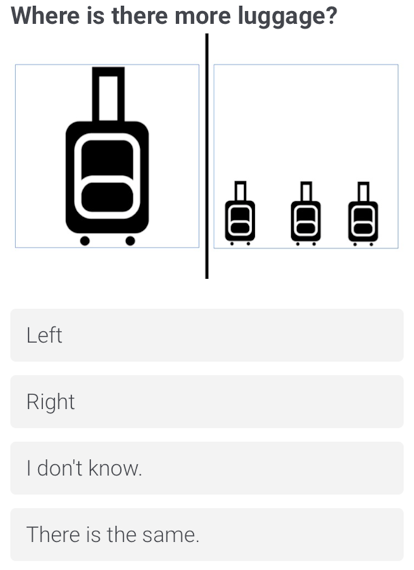
\includegraphics[width=1.8783in,height=2.5874in,width=\textwidth]{thomas-img1.png}
 
\end{styleStandard}


\begin{styleStandard}
\textit{Figure 2: A sample item from the PDT.}
\end{styleStandard}

\begin{styleStandard}
We administered a PDT in English to all groups, in which the following question was asked: \textit{Where is there more…?} Upon seeing two pictures — one large item/group, or three small items/groups as shown in Figure 2 \ —, this question forced participants to decide where there \textit{was more} of that noun item. Although Barner \& Snedeker (2005) posed the question \textit{Who has more…?} in the framing of their experiment, the present study tested the question: \textit{Where is there more…?}\footnote{\textstylefootnotereference{ }It might be objected that this presentation may pose the participants with an ungrammatical sentence, for instance \textit{Where is there more books?} We would like to emphasize here that we chose the use of the question \textit{Where is}, and to not change \textit{is} to \textit{are }when presented with plural items, because in Spanish/Catalan, there is one word/verb form that accounts for both \textit{there is} and \textit{there are}.} \ We changed the question in order to provide the participants a linguistic form that had similar structure throughout all three languages (e.g., English: \textit{Where are there more books?, }Spanish: \textit{¿Dónde hay más libros?, }Catalan: \textit{On hi ha més llibres?}). This change in wording was made so that the data could be usable in another study that compared English, Spanish, and Catalan. The participants always chose from the answers: \textit{left – right – I don’t know – There is the same.} As shown in Figure 2, the three small objects always showed a combined volume and surface area smaller than the large object. \ This allowed responses based on number to be distinguished from those based on mass or volume. 
\end{styleStandard}

\begin{styleStandard}
Table 5: Conditions for items in the PDT.
\end{styleStandard}

\begin{center}
\tablehead{}
\begin{supertabular}{|m{1.6809598in}|m{0.35525984in}|m{1.1254599in}|m{1.6941599in}|}
\hline
\textbf{Noun type} &
\textbf{\#} &
\textbf{Crosslinguistic Status} &
\textbf{Example item}\\\hline
Countable &
4 &
match &
\textit{Where is there more books?}\\\hline
Substance-uncountable &
4 &
match &
\textit{Where is there more salt?}\\\hline
Object-uncountable &
4 &
match &
\textit{Where is there more art?}\\\hhline{~---}
 &
4 &
mismatch &
\textit{Where is there more furniture}\\\hhline{~---}
Flexible (+ count) &
4 &
match &
\textit{Where is there more cakes?}\\\hline
Flexible (– count) &
4 &
match &
\textit{Where is there more cake?}\\\hline
\end{supertabular}
\end{center}
\begin{styleStandard}
Responses were rated by assigning a +1 if the picture with three small masses or items was chosen and a score of 0 if the picture of one large mass or item was chosen. A score of 0 was also assigned to \textit{They have the same} responses and an X was assigned to \textit{I don’t know}. The X scores were later excluded from data analysis. The scores were calculated and analyzed as percentages of individuation (e.g. total number of 1s divided by the total number of that noun type presented). In the PDT, as with the GJT, target sentences were created based on the five different noun types (countable, object-uncountable, substance-uncountable, – count flexible, and + count flexible). 
\end{styleStandard}

\begin{styleStandard}
Prior to participating in data collection, the participants completed two pre-participation questionnaires: a biodata and language use questionnaire and a quick English test. These questionnaires were web-based for all participants and administered via Qualtrics\footnote{ Qualtrics (2015). \textit{Qualtrics.} Accessed January – June 2015 at: http://www.qualtrics.com}. The NSs were sent the information via an email containing links to the experimental tasks, as well as a sociolinguistic survey. They were asked to complete the surveys within three weeks, and those who completed all the tasks were included in the data analysis. \ NNSs participants attended a data collection session in an on-campus computer lab during which they were administered the entire battery of instruments over the course of an hour and a half. The participants were offered a short break of 5-10 minutes between each of the data collection steps. 
\end{styleStandard}

\setcounter{listWWNumxxiileveli}{0}
\begin{listWWNumxxiileveli}
\item 
\begin{stylelsSectioni}
Results and discussion
\end{stylelsSectioni}


\setcounter{listWWNumxxiilevelii}{0}
\begin{listWWNumxxiilevelii}
\item 
\begin{stylelsSectionii}
Experiment 1: Results \& Discussion
\end{stylelsSectionii}

\end{listWWNumxxiilevelii}
\end{listWWNumxxiileveli}
\begin{styleStandard}
Experiment 1 allows us to address RQ1, that is, how the FI group would compare to the EMI and to NSs of English in their ability to grammatically recognize countable/uncountable noun distinctions, including object-uncountable noun, substance-uncountable nouns, and flexible noun types, and whether any influence from their two L1s would be revealed. \ In order to address this question, a series of one-way ANOVAs was run on the mean accuracy (scores out of 100) of the GJT with an alpha level set at 0.05. For the noun types tested, there was a statistically significant difference between groups as determined by one-way ANOVAs for countable nouns (\textit{F}(2,80) = 23.085, \textit{p} {\textless} .001), object-uncountable nouns (\textit{F}(2,80) = 96.938, \textit{p} {\textless} .001), flexible (+\textit{count}) nouns (\textit{F}(2,80) = 22.894, \textit{p} {\textless} .001), and flexible (–\textit{count}) nouns (\textit{F}(2,80) = 18.619, \textit{p} {\textless} .001). There was no statistical difference between groups for substance-uncountable nouns (\textit{F}(2,80) = 1.806, \textit{p} = .171). Average accuracy rates are presented in Table 6.
\end{styleStandard}

\begin{styleStandard}
\textit{Table 6: GJT Descriptive Statistics}
\end{styleStandard}

\begin{flushleft}
\tablehead{}
\begin{supertabular}{m{1.0254599in}|m{1.0226599in}m{1.0170599in}m{1.0163599in}m{-0.064140156in}m{1.0025599in}m{-0.052340157in}m{1.0150598in}}
\bfseries Group &
\bfseries Countable Nouns &
\bfseries Object-uncountable Nouns &
\bfseries Substance-uncountable Nouns &
\multicolumn{2}{m{1.0171599in}}{{\bfseries Flexible}

\bfseries (+\textit{ count}) Nouns} &
\multicolumn{2}{m{1.0414598in}}{{\bfseries Flexible}

\bfseries (\textit{{}- count}) Nouns}\\\hline
\mdseries NSs &
\mdseries 90.88 &
\mdseries 93.27 &
\multicolumn{2}{m{1.03096in}}{\mdseries 87.00} &
\multicolumn{2}{m{1.0289599in}}{\mdseries 96.15} &
\mdseries 91.35\\
\mdseries (\textit{N }= 26) &
\mdseries (9.05) &
\mdseries (8.23) &
\multicolumn{2}{m{1.03096in}}{\mdseries (15.15)} &
\multicolumn{2}{m{1.0289599in}}{\mdseries (5.88)} &
\mdseries (9.20)\\\hline
\mdseries FI Context &
\mdseries 83.71 &
\mdseries 46.97 &
\multicolumn{2}{m{1.03096in}}{\mdseries 80.30} &
\multicolumn{2}{m{1.0289599in}}{\mdseries 75.76} &
\mdseries 71.59\\
\mdseries (\textit{N = }33) &
\mdseries (19.13) &
\mdseries (11.49) &
\multicolumn{2}{m{1.03096in}}{\mdseries (17.50)} &
\multicolumn{2}{m{1.0289599in}}{\mdseries (17.10)} &
\mdseries (15.40)\\\hline
\mdseries EMI Context &
\mdseries 64.84 &
\mdseries 79.17 &
\multicolumn{2}{m{1.03096in}}{\mdseries 78.13} &
\multicolumn{2}{m{1.0289599in}}{\mdseries 73.44} &
\mdseries 76.69\\
\mdseries (\textit{N = }24) &
\mdseries (8.99) &
\mdseries (18.26) &
\multicolumn{2}{m{1.03096in}}{\mdseries (19.59)} &
\multicolumn{2}{m{1.0289599in}}{\mdseries (13.45)} &
\mdseries (11.36)\\\hline
\end{supertabular}
\end{flushleft}
\begin{styleStandard}
Looking at individual comparisons from a descriptive point of view, results of the GJT provided evidence that L2 English learners, from both the EMI and the FI, showed some difficulty in judging the grammaticality of constructions with countable and uncountable nouns in comparison to NSs of English. As visible in Table 6, the NSs performed with rates of accuracy nearly at ceiling across all the classes of nouns, with the exception of substance-uncountable nouns. All learner groups \ showed accuracy rates lower than those of the NS group in all categories. In Figure 3, it can be seen that EMI participants performed, on average, lower than those in a FI context with the exception of object-uncountable nouns (e.g. \textit{They have such beautiful furniture in their house} or \textit{There are many furnitures to choose from}) and flexible nouns used in a [– \textit{count}] context (e.g., \textit{John has some string in his bag}). 
\end{styleStandard}

\begin{styleStandard}
  [Warning: Image ignored] % Unhandled or unsupported graphics:
%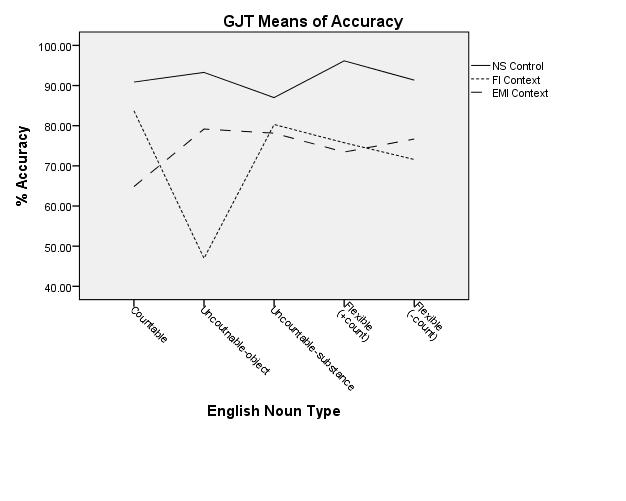
\includegraphics[width=4.4165in,height=3.072in,width=\textwidth]{thomas-img2.jpg}
  
\end{styleStandard}

\begin{styleStandard}
\textit{Figure 3: Profile plot of the participant groups’ performance on GJT}
\end{styleStandard}

\begin{styleStandard}
In order to test the significance of these differences among groups, post hoc tests using Tukey HSD were conducted. We will address each of the noun types individually. 
\end{styleStandard}

\begin{styleStandard}
As for countable nouns (e.g. judging the grammaticality of \textit{There are six dogs playing in the park} versus \textit{One third of the dog is in the garden}), a Tukey HSD post hoc test revealed that FI learners (\textit{M} = 83.71, \textit{SD} = 19.13) were significantly different (\textit{p }{\textless} .001) from EMI learners (\textit{M} = 64.84, \textit{SD} = 8.99). The FI learners were not significantly different from the NSs (\textit{M} = 90.87, \textit{SD} = 9.05, \textit{p} = .131), while the EMI leaners were (\textit{p} {\textless} .001). 
\end{styleStandard}

\begin{styleStandard}
For \ object-uncountable nouns (e.g. \textit{They have such beautiful furniture in their house} vs. \textit{There are many furnitures to choose from}), the FI learners had means of accuracy below 50\% (\textit{M} = 46.97, \textit{SD} = 11.49), which was much lower than the EMI learners (\textit{M} = 79.17, \textit{SD} = 18.26). A Tukey HSD post hoc analysis showed that this difference \ was significant with \textit{p} {\textless} .001. When comparing the NNSs to NSs (\textit{M} = 93.27, \textit{SD} = 8.83), both learning contexts performed significantly lower (\textit{p }{\textless} .001 for both groups). 
\end{styleStandard}

\begin{styleStandard}
In regard to substance-uncountable nouns, the NSs performed lower than 90\% overall (\textit{M} = 87.00, \textit{SD} = 15.15), and both NNS groups’ accuracy was quite close to this level. Thus, the difference with learner groups was not significant : \textit{p }= .314 for the FI learners and \textit{p} = .178 for the EMI learners. The FI learners were on average slightly more accurate (\textit{M} = 80.30, \textit{SD} = 17.50) than the EMI learner group (\textit{M} = 78.13, \textit{SD} = 19.59), although this difference was not significant (\textit{p }= .888). 
\end{styleStandard}

\begin{styleStandard}
The data concerning flexible nouns do not show any relevant difference between the experimental groups. For flexible nouns presented with count syntax, henceforth flexible (\textit{+count}), the NS group performed at high rates of accuracy (\textit{M} = 96.15, \textit{SD} = 5.88). The EMI learners performed with the lowest mean accuracy (\textit{M} = 73.44, \textit{SD} = 13.45), while the FI learners performed a little higher (\textit{M} = 75.76, \textit{SD} = 17.10). The difference between the two experimental groups was not significant (\textit{p }= .796), although they both performed significantly lower than the NSs (\textit{p }{\textless} .001 for both groups).
\end{styleStandard}

\begin{styleStandard}
Flexible nouns presented in uncountable syntax, flexible (\textit{– count}), present a different picture, with the EMI learners achieving slightly higher rates of accuracy (\textit{M} = 76.69, \textit{SD} = 11.36) than the FI learners (\textit{M} = 71.59, \textit{SD} = 15.40), although this difference was not significant (\textit{p }= .291). The NSs achieved significantly higher rates of accuracy (\textit{M} = 91.35, \textit{SD} = 9.20) than both of the experimental groups (\textit{p }{\textless} .001 for both groups). 
\end{styleStandard}

\begin{styleStandard}
To summarize, the first research question explored the linguistic ability of both the FI and EMI experimental groups of NNSs in comparison to NSs in their ability to recognize grammatical and ungrammatical uses of countable/uncountable noun distinctions in English. The results of the GJT provided evidence that the NNSs, both FI and EMI, showed some difficulty, although not significant in all noun types,. In comparison to NSs, differences were significant in the case of countable nouns for the EMI group; for both groups in the case of object-uncountables, and non-significant for substance-uncountable and for flexible nouns in countable contexts. They were again significant for flexible nouns in uncountable contexts. 
\end{styleStandard}

\begin{styleStandard}
When comparing learning contexts, the FI group performed significantly higher than the EMI group with regard to countable nouns, while they performed only slightly higher with substance-uncountable nouns and flexible (+count). The EMI group did perform slightly better than the FI group with regard to object-uncountable nouns and flexible (–count) nouns. \ Thus, there was no clear trend favoring either FI or EMI. It must be remembered that the EMI group had around seven times more hours of exposure per week than the FI group (15/20 versus 3, respectively), potentially including many contexts for using these classes of nouns. On the other hand, the FI group had received explicit instruction, and more precisely 4 hours, on countability issues. Consequently, it can be stated that the contrast between both groups in terms of quantity and quality of exposure also results in mixed, or asymmetric, comparative results. 
\end{styleStandard}

\begin{listWWNumxxiileveli}
\item 
\setcounter{listWWNumxxiilevelii}{0}
\begin{listWWNumxxiilevelii}
\item 
\begin{stylelsSectionii}
Experiment 2: Results \& Discussion
\end{stylelsSectionii}

\end{listWWNumxxiilevelii}
\end{listWWNumxxiileveli}
\begin{styleStandard}
\ Experiment 2 allows us to address RQ2: to what extent the judgments elicited with the PDT were based on linguistic or extra-linguistic knowledge and whether there are any differences among EMI and FI students and L1 English speakers. \ 
\end{styleStandard}

\begin{styleStandard}
We will now look at the results of the PDT in English and compare the EMI learners to the FI learners and the NSs. Results will be reported as percentages of individuation based on English noun type. It should be borne in mind that answers were scored by awarding +1 point if the participant chose the picture with three small masses or items and a score of 0 if the picture chosen represented a large mass or item. To calculate percentages of individuation, the positive numbers were added together and then divided by the total number of items in that category, which was always 4. In other words, if a participant chose the picture of three small items for \textit{books, dogs, }and \textit{doors}, but not for \textit{windows}, then they would receive a score of 3. That score was then divided by 4 to get a percentage of indivudation as 75\%. Likewise, one would predict lower percentages of individuation for uncountable-substance and flexible (–\textit{count}) items. For example, if a participant selected the picture of three small piles for \textit{cake}, but the larger mass for \textit{paper, stone, }and \textit{chocolate}, then they would receive a score of 1 out of four. That would be converted into a percentage of individuation of 25\%. In short, one would expect high percentages of individuation for countable, object-uncountable, and flexible (+\textit{count}) nouns since those nouns are countable and, therefore, refer to objects that can be individuated and low percentages of individuation for substance-uncountable and flexible (–\textit{count}) nouns since those nouns are uncountable and, therefore, refer to masses of substances. 
\end{styleStandard}

\begin{styleStandard}
In order to address this research question, a series of one-way ANOVAs was run on the mean percentages of individuation (scores out of 100) of the PDT, with an alpha value set at 0.05. For the noun types tested, there was no statistically significant difference between groups as determined by one-way ANOVA for countable nouns (\textit{F}(2,80) = .029, \textit{p} = .972), object-uncountable nouns (\textit{F}(2,80) = 1.181, \textit{p} = .312), or substance-uncountable nouns (\textit{F}(2,80) = .189, \textit{p} = .828). As for flexible nouns, there was no statistical difference found for flexible (+\textit{count}) nouns (\textit{F}(2,80) = .115, \textit{p} = .892) nor flexible (–\textit{count}) nouns (\textit{F}(2,80) = .078, \textit{p} = .925). Individuation rates are provided in Table 7.
\end{styleStandard}

\begin{styleStandard}
\textit{Table 7: PDT Descriptive Statistics}
\end{styleStandard}

\begin{flushleft}
\tablehead{}
\begin{supertabular}{m{1.0538598in}|m{0.97685987in}m{0.9816598in}m{-0.062040158in}m{1.3080599in}m{0.95665985in}m{-0.055840157in}m{0.95525986in}}
\bfseries Group &
\bfseries Countable Nouns &
\bfseries Object-uncountable Nouns &
\multicolumn{2}{m{1.32476in}}{\bfseries Substance-uncountable Nouns} &
{\bfseries Flexible }

\bfseries (+\textit{ count}) Nouns &
\multicolumn{2}{m{0.97815984in}}{{\bfseries Flexible}

\bfseries (\textit{{}- count}) Nouns}\\\hline
\mdseries NSs &
\mdseries 96.15 &
\multicolumn{2}{m{0.99835986in}}{\mdseries 85.58} &
\mdseries 33.65 &
\multicolumn{2}{m{0.97955984in}}{\mdseries 93.27} &
\mdseries 52.88\\
\mdseries (\textit{N }= 26) &
\mdseries (15.32) &
\multicolumn{2}{m{0.99835986in}}{\mdseries (20.22)} &
\mdseries (42.98) &
\multicolumn{2}{m{0.97955984in}}{\mdseries (20.69)} &
\mdseries (42.03)\\\hline
\mdseries FI Context &
\mdseries 96.21 &
\multicolumn{2}{m{0.99835986in}}{\mdseries 76.52} &
\mdseries 27.27 &
\multicolumn{2}{m{0.97955984in}}{\mdseries 91.67} &
\mdseries 56.82\\
\mdseries (\textit{N = }33) &
\mdseries (11.04) &
\multicolumn{2}{m{0.99835986in}}{\mdseries (25.72)} &
\mdseries (36.10) &
\multicolumn{2}{m{0.97955984in}}{\mdseries (18.40)} &
\mdseries (38.16)\\\hline
\mdseries EMI Context &
\mdseries 96.88 &
\multicolumn{2}{m{0.99835986in}}{\mdseries 81.25} &
\mdseries 30.21 &
\multicolumn{2}{m{0.97955984in}}{\mdseries 93.75} &
\mdseries 54.17\\
\mdseries (\textit{N = }24) &
\mdseries (8.45) &
\multicolumn{2}{m{0.99835986in}}{\mdseries (20.19)} &
\mdseries (40.36) &
\multicolumn{2}{m{0.97955984in}}{\mdseries (11.06)} &
\mdseries (37.35)\\\hline
\end{supertabular}
\end{flushleft}
\begin{styleStandard}
Looking at individual comparisons from a descriptive point of view, results of the PDT provided evidence that L2 English learners, from both the EMI and the FI groups, showed very similar patterns of individuation (or quantificational judgments) to NSs of English. \ Table 7 shows the means of individuation for all the groups. \ 
\end{styleStandard}

\begin{styleStandard}
Given the very similar results, post hoc tests using Tukey HSD showed no statistical differences among groups, with all p values higher than .715 
\end{styleStandard}

\begin{styleStandard}
These strong similarities among groups deserve some comments. The most striking, and perhaps unexpected, is that regarding object-uncountable nouns (e.g., \textit{Where is there more furniture?}). English native speakers’ individuation rate was the highest (\textit{M} = 85.58), followed by EMI learners \ (\textit{M} = 81.25) and FI learners (\textit{M} = 76.52). This means that, even though in English some nouns are uncountable only (e.g. \textit{luggage}, which may be grammaticalized as countable in Catalan/Spanish, i.e. \textit{equipajes}), judgments seem to be based in all cases on semantics (the mental representation of individual objects) rather than on grammar (the mass- vs. count-noun distinction). This provides further evidence for Barner \& Snedeker’s (2005) claim that, for object-uncountable nouns, English speakers rely more on semantics than on their language’s grammar. 
\end{styleStandard}

\begin{styleStandard}
Another rather unexpected finding was the proportion of participants who selected the individuating option for substance-uncountable nouns. Although all groups perceived these stimuli (such as \textit{water}) to refer more to masses rather than to individuals, and thus tended to select the picture with the big object rather than the one with several small ones, about one third of the answers seemed to interpret some of the substance-uncountable nouns as being [+ \textit{individual}] (e.g., \textit{milk }and \textit{water}). This\textit{ }could be attributed to the fact that, in the PDT, the uncountable substances which were liquid, appeared as “cups” of those substances and therefore might have been interpreted as [+ \textit{individual}].
\end{styleStandard}

\begin{styleStandard}
A similar phenomenon was observed for flexible nouns. While all three groups consistently interpreted flexible nouns in terms of individuation in [+ \textit{count}] syntactic contexts (e.g. \textit{Where is there more cakes?}), in [– \textit{count}] contexts (e.g. \textit{Where is there more cake?}) about 50\% of the responses individuated (e.g. chose the picture of three small \textit{cakes}), while the other 50\% did not individuate (e.g. chose the picture of one large \textit{cake}). As with the substance-uncountable nouns, it is possible that the pictures that represented flexible nouns in the PDT did not provide appropriate interpretations of mass representations (e.g. a large cake instead of three small cakes). Thus, our experiment provides only partial evidence that syntax drives the individualized interpretation of flexible nouns presented in a [– \textit{count}] context, as was found by Barner \& Snedeker (2005).
\end{styleStandard}

\begin{listWWNumxxiileveli}
\item 
\begin{stylelsSectioni}
Conclusions
\end{stylelsSectioni}

\end{listWWNumxxiileveli}
\begin{styleStandard}
The present study evaluated the acquisition of English by Spanish/Catalan speakers from two different EFL learning contexts, conventional FI and EMI, to gauge their respective impact on learners’ target language abilities vis-à-vis countability. To do so, we followed Barner \& Snedeker (2005), who used a similar PDT to investigate English-speaking children’s developmental patterns and adults’ representations of countable-uncountable noun semantics, in addition to a GJT based on 100 items. No previous studies have investigated this phenomenon in NNSs, specifically from a bilingual background, in different learning contexts, FI and EMI, and with a crosslinguistic perspective. 
\end{styleStandard}

\begin{styleStandard}
Regarding RQ1, which looked into the EMI and FI participants’ ability to recognize grammatical and ungrammatical uses of countable/uncountable noun distinctions in English, the results of the GJT provided evidence that the NNSs of English showed some difficulty, although not significant in all noun types, with regards to the judgments of countable and uncountable noun distinctions when used in grammatical and ungrammatical contexts in comparison to the NSs, irrespective of whether they were studying English in a FI or EMI context. Differences with native speakers were significant in the case of countable nouns for the EMI group, in favor of the NSs; for both the FI and the EMI groups in the case of uncountable-objects, in favor of the NSs, and non-significant for uncountable-substance and for flexible nouns in both countable and uncountable contexts. There were no clear and consistent differences between the EMI and the FI groups, which shows that both programs seem to have similar effects on this dimension of language performance, despite their obvious difference as regards amount of input and instructional approach (implicit vs. explicit).
\end{styleStandard}

\begin{styleStandard}
Regarding RQ2, which enquired into the participants’ judgments of individuation for different noun types, results have shown a large amount of similarity across groups \ when comparing the PDT data collected from NSs and NNSs of English. Most importantly, the fact that English L2 learners had similar response patterns as NSs regarding object-uncountable nouns, which receive different grammatical encodings in English versus Catalan/Spanish, supports Barner \& Snedeker’s (2005) theory that mental representations of object-uncountable nouns do represent individual objects, and provide additional evidence that they do not seem to differ across speakers of different languages, regardless of how these encode them in the grammar (as countable or uncountable nouns). Our results also agree with Barner \& Snedeker’s (2005) conclusion that flexible nouns are interpreted based on the syntactic context in which they occur, although in our data the difference between [+ count] and [– count] contexts was not as clear-cut as in their original experiments. 
\end{styleStandard}

\begin{styleStandard}
This chapter and these conclusions, though, do not come without consequences and limitations. We do believe that the presentation of the pictures makes the task to some extent unnatural, although this is true of many controlled experimental conditions. We also believe that expanding the research to all levels of learners would give some better insight into the acquisition process of countable and uncountable nouns. 
\end{styleStandard}

\begin{stylelsSectioni}
Acknowledgments
\end{stylelsSectioni}


\begin{styleStandard}
We would like to thank Eloi Puig-Mayenco and Jennifer Ament for their help in participant recruitment and data collection, as well as their valuable comments throughout the writing process.
\end{styleStandard}

\begin{stylelsSectioni}
References
\end{stylelsSectioni}


\begin{styleStandard}
Barner, David \& Snedeker, Jesse. 2005. Quantity judgments and individuation: evidence that mass nouns count. \textit{Cognition} 97. 41-66.
\end{styleStandard}


\begin{styleStandard}
Bloom, Paul \& Keleman, Deborah. 1995. Syntactic cues in the acquisition of collective nouns. \textit{Cognition} 56. 1-30.
\end{styleStandard}


\begin{styleStandard}
Bruyne, Jacques de. 1995. \textit{A comprehensive Spanish grammar}. Cambridge, MA: Blackwell.
\end{styleStandard}


\begin{styleStandard}
Butt, John \& Benjamin, Carmen. 2004. \textit{A new reference grammar of modern Spanish}. London: E. Arnold.
\end{styleStandard}


\begin{styleStandard}
Chaudron, Craig. 2003. Data collection in SLA research. In Doughty, Catherine J. \& Long, Michael. H. (eds.), \textit{The handbook of second language acquisition}, 762-828. Malden, MA: Blackwell.
\end{styleStandard}


\begin{styleStandard}
Coleman, James A. 2006. English-medium teaching in European higher education. \textit{Language Teaching} 39(1). 1–14.
\end{styleStandard}


\begin{styleStandard}
Cowan, Ron \& Hatasa, Yukiko Abe. (1994). Investigating the validity and reliability of native speaker and second language learner judgments about sentences. In Tarone, Elain E. \& Gass, Susan M. \& Cohen, Andrew D. (Eds.), \textit{Research methodology in second language acquisition}, 287-302. Hillsdale: Lawrence Erlbaum.
\end{styleStandard}


\begin{styleStandard}
Cowart, Wayne. 1997. Experimental syntax: Applying objective methods to sentence judgments. Thousand Oaks: SAGE Publications, Inc.
\end{styleStandard}


\begin{styleStandard}
Dafouz, Emma \& Guerrini, Michele C. (eds.) 2009. CLIL across educational levels: Experiences from primary, secondary and tertiary contexts. Madrid: Santillana Educación.
\end{styleStandard}


\begin{styleStandard}
Ellis, Rod. 2010. Second language acquisition, teacher education and language pedagogy. \textit{Language Teaching} 43. 182-201.
\end{styleStandard}


\begin{styleStandard}
Gass, Susan M. 1994. Second language acquisition: An introductory course. New York: Routledge.
\end{styleStandard}


\begin{styleStandard}
Ionin, Tania \& Zyzik, Eve. 2014. Judgment and interpretation tasks in second language research. \textit{Annual Review of Applied Linguistics }34. 1-28.
\end{styleStandard}


\begin{styleStandard}
Izumi, Shinichi. 2013. Focus on Form (FonF). In Robinson, Peter (ed.), \textit{The Routledge encyclopedia of second language acquisition, }244-249. New York: Routledge.
\end{styleStandard}


\begin{styleStandard}
Landman, Fred. 2011. Count nouns – mass nouns, neat nouns – mess nouns. In Skilters, Jurgis (ed.), \textit{The Baltic International Yearbook of Cognition, Logic and Communication} 6. 1-67.
\end{styleStandard}


\begin{styleStandard}
Leech, Geoffrey \& Svartvik, Jan. 1975. \textit{A communicative grammar of English}. London: Longman.
\end{styleStandard}


\begin{styleStandard}
Norris, John \& Ortega, Lourdes. 2003. Defining and measuring SLA. In Doughty, Catherine J. \& Long, Michael H. (eds.), \textit{The handbook of second language acquisition}, 716-761. Malden, MA: Blackwell.
\end{styleStandard}


\begin{styleStandard}
Pérez-Vidal, Carmen. 2009. The integration of content and language in the classroom: a European approach to education (the second time around). In Dafouz, Emma. \& Guerrini, Michele C. (eds.), \textit{CLIL across educational levels: Experiences from primary, secondary and tertiary contexts}, 25-40\textit{. }Madrid: Santillana Educación.
\end{styleStandard}


\begin{styleStandard}
Pérez-Vidal, Carmen. 2011. Language acquisition in three different contexts of learning: Formal instruction, study abroad, and semi-immersion (CLIL). In\textit{ }Ruiz de Zarobe, Yolanda, Manual Sierra, Juan, \& Gallardo del Puerto, Francisco. (eds.),\textit{ Content and foreign language integrated learning, }103-129. Bern: Peter Lang.
\end{styleStandard}


\begin{styleStandard}
Wächter, Bernd \& Maiworm, Friedhelm. (eds.). 2014. English-taught programmes in European higher education: The state of play in 2014. Bonn: Lemmens Medien GmbH.
\end{styleStandard}


\begin{styleStandard}
Wheeler, Max \& Yates, Alan \& Dols, Nicolau. 1999. \textit{Catalan: A comprehensive grammar}. New York: Routledge.
\end{styleStandard}

\end{document}
